\section{Einleitung}
Ähnlich wie der Lebensraum der Fische auf das Wasser begrenzt ist, so ist unser 
Lebensraum begrenzt auf das Universum.
Weiss ein Fisch, wie das Meer von unserem Blickpunkt aus aussieht?
Wahrscheinlich nicht, wieso sollte ihn das auch interessieren?
Da wir aber keine Fische sind, ist es nur natürlich sich zu fragen, wie das 
Universum von Aussen betrachtet, aussieht.
Um die Frage nach der Form des Universums beantworten zu können, werden wir uns 
im folgenden Kapitel mit dem kosmischen Mikrowellenhintergrund befassen.

\subsection{Der kosmische Mikrowellenhintergrund}
Glaubt man der Theorie des Big-Bang, (was wir im folgenden tun wollen) so waren 
der Druck und die Temperaturen in den ersten ca. 380'000 Jahren nach dem 
Big-Bang so, dass Atome nicht existieren konnten.
Die gesamte Materie bestand stattdessen aus ionisiertem Plasma, welches sehr 
effizient darin war, Strahlung zu streuen (dieser Effekt ist unter 
Thomson-Streuung bekannt).
Das einzige was wir heute sehen, wenn wir weit genug in der Zeit zurückblicken,
ist eine Art opaker Nebel (siehe Abbildung \ref{fig:radiation_scattering}).
% TODO replace with better image
\begin{figure}
	\centering
	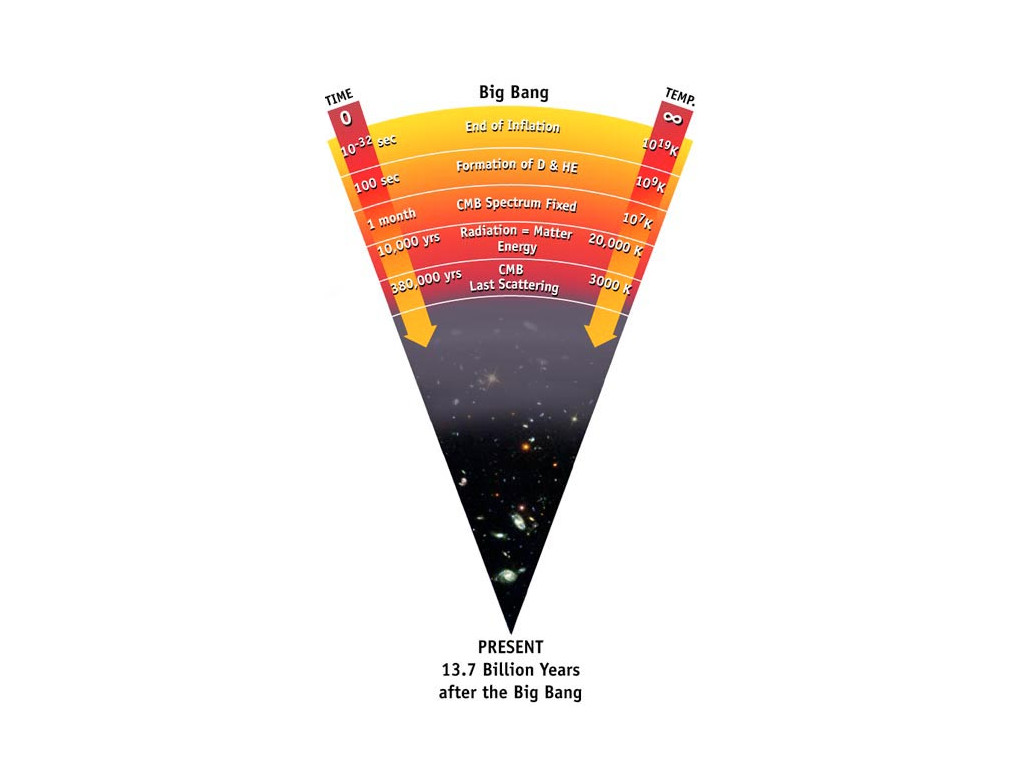
\includegraphics[width=\linewidth]{cmb/images/radiation_scattering.jpg}
	\caption{Entstehung des Universums im Zeitverlauf. Beim ``Last Scattering'' 
	Prozess wurde das Universum sichtbar}
	\label{fig:radiation_scattering}
\end{figure}

Im Verlauf der nächsten 380'000 Jahre (relativ gesehen ein sehr kurzer 
Zeitraum) und der damit verbundenen Ausdehnung des Universums sanken Druck und 
damit die Temperatur im Universum stark, auf etwa $3700 \text{K}$.
Nun waren die Bedingungen erfüllt, dass sich Protonen und Elektronen zu 
Wasserstoffatomen verbinden konnten, wie in Abbildung \ref{fig:recombination} 
zu sehen ist. Die Zeit in der sich die ersten Atome bildeten, ist auch als 
Rekombination bekannt (siehe Abschnitt 12.2).

Nach dieser Rekombination gab es keine freien Elektronen mehr, wodurch die 
Photonen nicht mehr durch Thomson-Streuung abgelenkt wurden.
Den Photonen war es jetzt endlich möglich, dem Nebel des frühen Universums zu 
entkommen und sich frei zu bewegen.
% Bild verkleinern
\begin{figure}
	\centering
	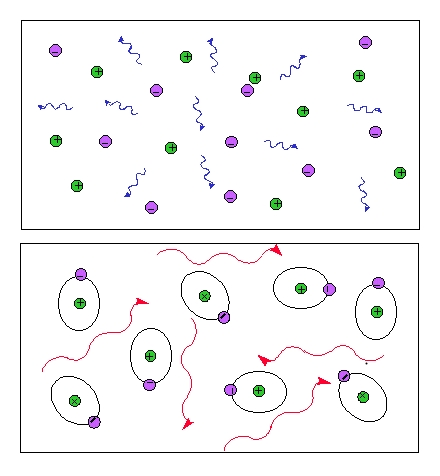
\includegraphics[scale=0.5]{cmb/images/recombination.jpg}
	\caption{Protonen, Neutronen und Photonen vor (oben) und nach (unten) der Rekombination. Vor der 
		Rekombination vertstreuten die freien Elektronen die Photonen. Danach waren die Elektronen gebunden
		und die Photonen konnten sich frei bewegen.}
	\label{fig:recombination}
\end{figure}
\ref{recombination}
Die kosmische Mikrowellenhintergrundstrahlung ist eine Aufzeichnung der Photonen zum 
Zeitpunkt der Rekombination und verfügt über das thermische Spektrum einer Schwarzkörperstrahlung.

Abbildung \ref{fig:blackbody_spectrum} zeigt, dass Temperatur und Wellenlänge einer Schwarzkörperstrahlung proportional sind.
Aufgrund dieser Proportionalität lässt sich genau vorhersagen, welche Temperatur der kosmische Mikrowellenhintergrund zu welcher Zeit hatte.
\begin{figure}
	\centering
	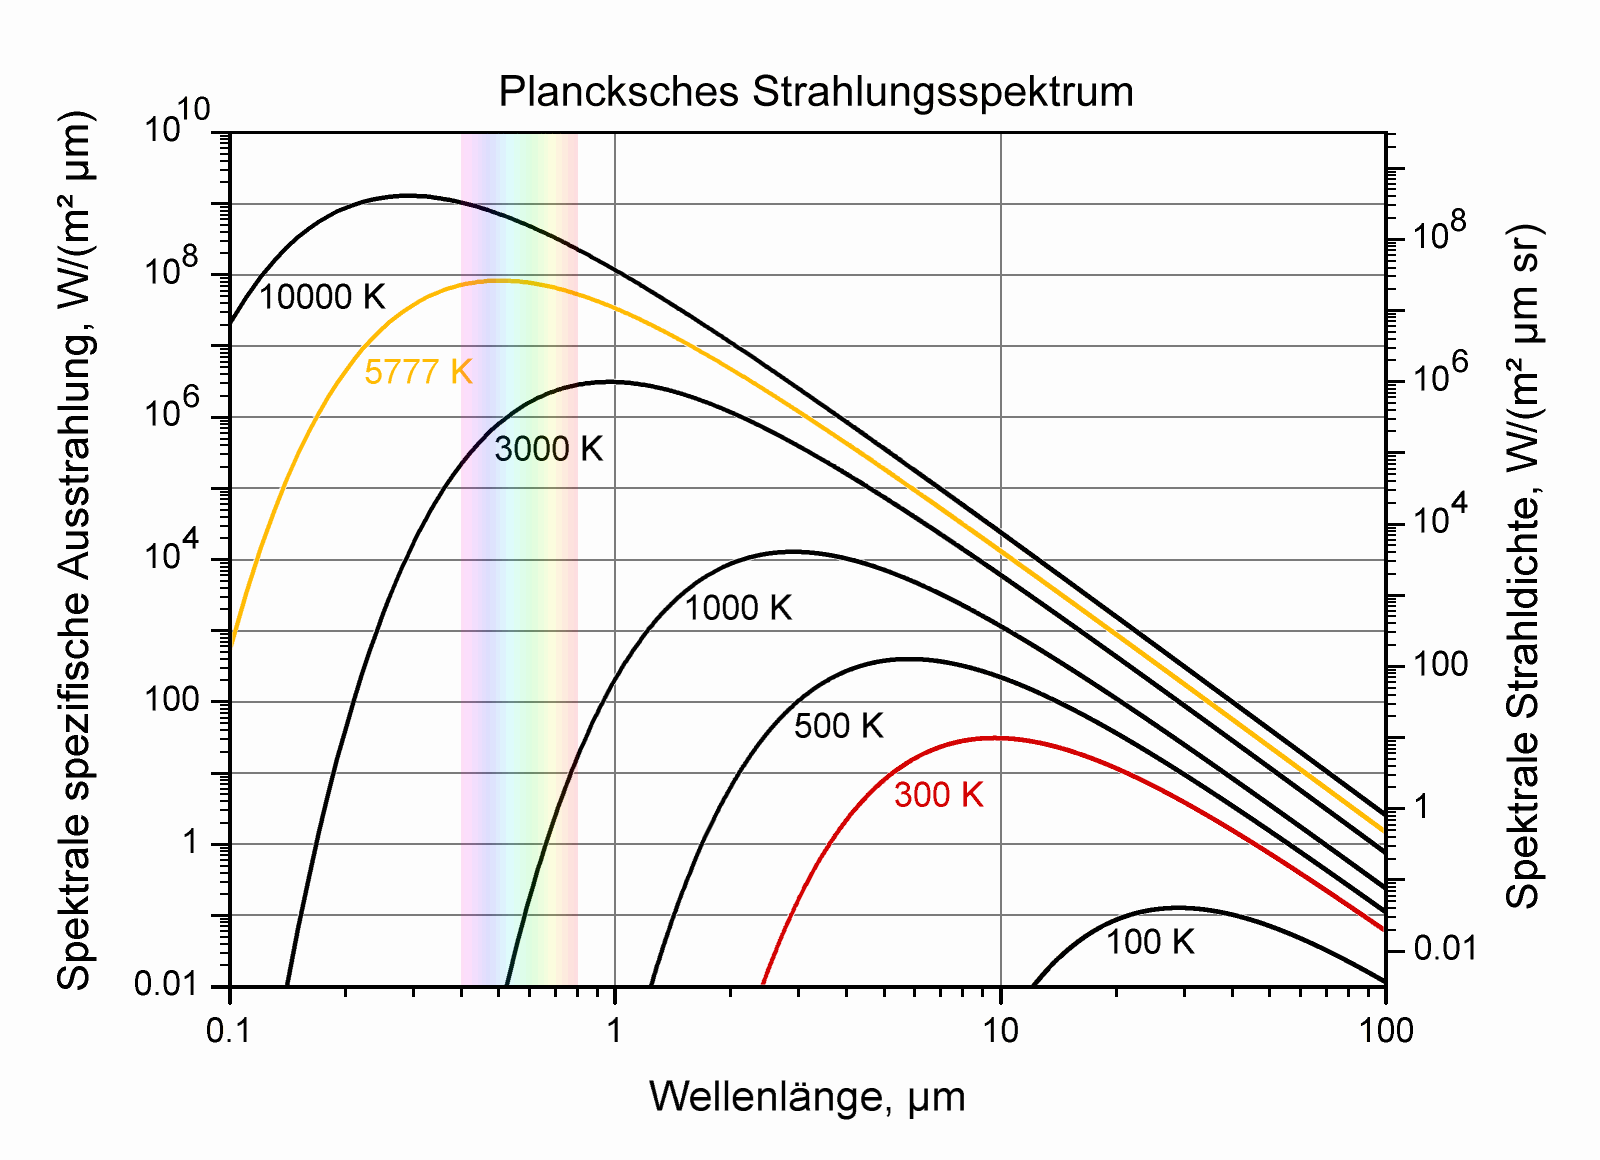
\includegraphics[width=\linewidth]{cmb/images/blackbody_spectrum.png}
	\caption{Plancksche Strahlungsspektren für verschiedene Temperaturen in doppeltlogarithmischer Auftragung}
	\label{fig:blackbody_spectrum}
\end{figure}
(Dieser Tatsache ist essentiell für die spätere Entdeckung der Strahlung).
\ref{CMB_intro}
